\section{System Designs}
In this section, all of the design aspects of this system have been detailed and justified. 

\subsection{UI Design}
As the purpose of this project was to aid in the accessibility and usability of fuzzy logic, to users of all skill levels, the design of the user interface was extremely important. The difference between a good piece of software, and a great piece of software, can easily be the interface they provide. In fact, the entire reason that FuzzyToolkitUoN is an inadequate piece of software for specifying fuzzy sets, is it's interface, and this is the exact thing this project aims to overcome. There were two main iterations to the user interface design, the first was a simple attempt to include all information on the page, in an easily viewable format. The second iteration was a refinement of the first stage, in which design principles were applied, and feedback was gathered from potential end users. \ \\
\ \\
It is worth noting that all the different tasks of constructing a fuzzy system (specifying inputs, specifying outputs, specifying rules, evaluating the system, and file input and output) are distinct tasks, and there is no reason for them to be together at any point. This is why, regardless of design, these tasks are all separated and are on different pages, or tabs, of the website. Further to this, the designs presented below cover only the input variable creation page and the rule creation page, as the output creation page is an exact replica of the input variable creation page, and the remaining pages or tabs of the website do not require much level of design, as they are relatively small.

\subsubsection{First Iteration}
\begin{figure}[ht!]
\begin{center}
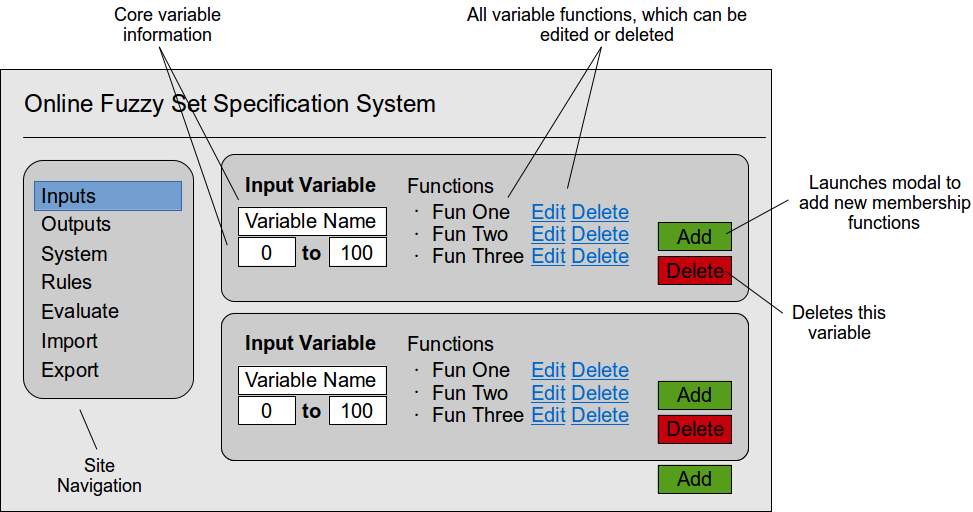
\includegraphics[width=0.9\textwidth]{images/firstItInputs}
\end{center}
\vspace{-2mm}
\caption{The first iteration of the design of the input creation page}
\label{fig:design-firstIterationInputs}
\vspace{-1mm}
\end{figure}
\noindent 
The first iteration of the input creation page listed the navigation to the left hand side of the page, as this is a standard positioning for navigation \cite{mccarthy2004could}, and the users would, most likely, be accustomed to this. \ \\
\ \\
The separation of different tasks to different sections of the website is very important for the construction of a fuzzy system, as there are many individual elements, and a lack of separation of these would cause a great deal of confusion for the user, as there would be a huge number of elements on the screen at one time.\ \\
\ \\
The design displays the core information of the variable on the far left (including name and range), as this is where the user's eye would fall first. The next set of information (the functions contained within the variable), are displayed further to the right, as the user would look to here after reading the initial information. The users have the option to edit or delete any function that they have created, granting them complete freedom over the system and everything they do within it. They also have the option to add a new membership function (which is a green button, to represent creation, which brings up a modal window to be used to construct the membership function), or delete the current variable (which is a red button, to represent destruction). \ \\
\ \\
This design uses long horizontal representations of the variables, so a large number of them can be on the screen at the same time, as they take up little vertical space. This means the users can view many of their variables at the same time, and make edits as necessary. Colour is used sparingly throughout the page, so that it can be used effectively for highlighting important information or elements, so they are easily visible to the user.

\begin{figure}[ht!]	
\begin{center}
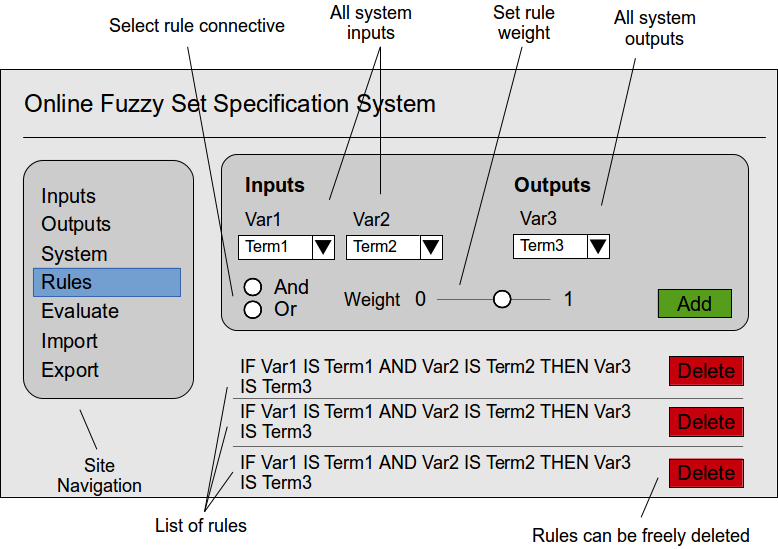
\includegraphics[width=0.825\textwidth]{images/firstItRules}
\end{center}
\vspace{-5mm}	
\caption{The first iteration of the design of the rule creation page}
\label{fig:design-firstIterationRules}
\end{figure}
\noindent 
The rule creation page also follows a horizontal theme, which is especially effective for the rules, as there could potentially be a long list of them. The creation of the rules, and their displaying, are two clearly distinct segments to the page, which means there is no confusion between the two, and the process remains a simple one. In keeping with the standards of the previous page, the ``Add'' button is coloured green, to represent creation, and the ``Delete'' buttons present by each rule are coloured red, to represent destruction. These clear colour separations are useful to the user, as they do not even need to read a button to gain an understanding of what it will do \cite{cyr2010colour}, and they can be more careful to not make mistakes.\ \\
\ \\
\vspace{-1mm}
As can be seen, the navigation and header of the rule creation page are the same as those on the input creation page, which promotes a consistent style amongst the pages, and helps to remind the user they are still within the same system, even if they are completing a different task. 


\subsubsection{Second Iteration}

\begin{figure}[ht!]
\begin{center}
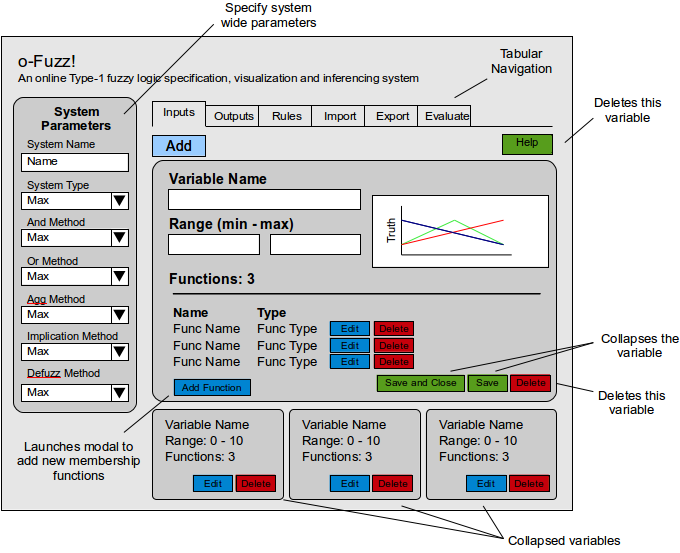
\includegraphics[width=1.1\textwidth]{images/secondItInputs}
\end{center}
\vspace{-6mm}
\caption{The second iteration of the design of the input creation page}
\label{fig:design-secondIterationInputs}

\end{figure}
\noindent

\noindent 
The second iteration of the input creation page design includes many improvements over the first iteration. Specifically, this second iteration dealt with the issues the first iteration presented, and had well known and well documented usability heuristics and design principles applied to it, to ensure optimality. \ \\
\ \\
One of the largest changes to the design was the re-working of the navigation to be entirely tabular, and to replace the old navigation area with system wide parameters segment. This tabbing helps to split the different tasks of the system in an intuitive manner, as most users are familiar with the concept of tabs, due to their popularity within internet browsers \cite{huang2010parallel}. The system wide parameters are now displayed in place of the old navigation, which means they can be changed, regardless of the tab the user is on. This is especially convenient when the user comes to evaluate the system, as it makes tuning much quicker, and all permutations of parameters can be evaluated with ease.\ \\
\ \\
The overall structure and displaying of the variables has also been drastically changed in this second iteration of design. The reason for this was that, whilst the old design promoted a large number of variables on the screen at any one time, this would severely increase the cognitive load on the user, and they could quickly become confused.\ \\
\ \\
The new design works by having expandable and collapsible variables. When in the collapsed view, the variable takes up a much smaller space, displaying only key information, and in the expanded view, all of the information of the variable is present (like in the previous design). The ideal number of elements on a page is 7$\pm$2 \cite{miller1956magical}, which can easily be exceeded with these new collapsed variables. However, the reason this design works, is because when the variable is collapsed, the user feels like it is completed, and they no longer need to concern themselves with it. So whilst this new design may look more cluttered, it significantly helps to reduce the cognitive load of the user, as they can create a variable, and then essentially forget about it.\ \\
\ \\
To fit with the consistency of the other pages, the buttons for the editing and deletion of membership functions have also been changed. The edit button is now blue, which is the system wide colour for editing, and the delete buttons are now red, the system wide colour for deletion. This keeps the website consistent, and makes the functionality of these buttons easily identifiable.\ \\
\ \\
Some other smaller changes include the moving of the ``Add'' button from the bottom right of the page, to the top left. so that it would not constantly move down the page as variables were added, as a moving button can be frustrating and confusing for some users. Another change is the addition of a short name for the software, with a longer tag-line underneath this, at the top of the page. This shortened title allows for users to refer to system with ease, allowing them to search for help for the system if necessary, and simply discuss the system with other potential users. The longer tag-line allows for a brief description of the system, so the user knows whether it will be able to accomplish the tasks they have set out to achieve. A graphical representation of each variable is now also displayed in the expanded view, allowing the user to quickly interpret how their system is progressing, and whether it looks as they expected. This is a very powerful tool, as users will be able to spot errors much sooner than if this were not present.


\begin{figure}[ht!]
\begin{center}
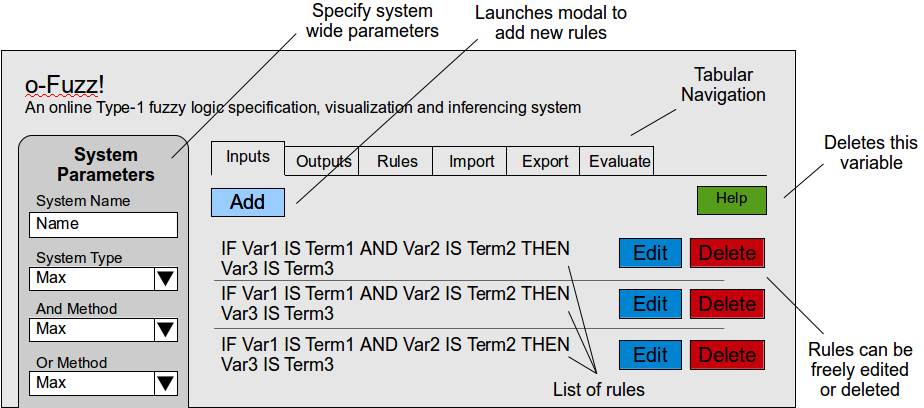
\includegraphics[width=0.95\textwidth]{images/secondItRules}
\end{center}
\caption{The second iteration of the design of the rule creation page}
\label{fig:design-secondIterationRules}
\end{figure}
\noindent 
The rules creation page also received heavy changes in the second iteration. The first of these was the inclusion of certain features that were not present in the first design, but were necessary for the functioning of the program. For instance, the ability to edit rules once they had been created, the ability to create negated terms (for instance, ``If food is \textit{not} good'') and the addition of the help button to the page.\ \\
\ \\
However, the biggest change is the removal of the ability to create rules on this initial page. Instead, as with the creation of membership functions, this has been moved into a separate window that is launched when the user clicked the ``Add'' button. This reduces the clutter on the page, and means the rule creation functionality is only accessed when the user requires it (helping to reduce cognitive load on the user).\ \\
\ \\
In addition, an extra feature was included in the form of a rule table that could be displayed if the user was using a system with two inputs, and one output (a relatively common set up for a fuzzy system). If this were the case, the table would be displayed, mapping the inputs to the outputs, in an intuitive graphical manner, an example of which can be seen in figure \ref{fig:ruleTable}.

\begin{figure}[ht!]
\begin{center}
\begin{tabular}{cl|lll}
\multicolumn{2}{c|}{} & \multicolumn{3}{c}{Body Temperature} \\
\multicolumn{2}{c|}{   }	& Low & Medium & High \\
\hline
\multirow{3}{10mm}{Heart Rate}	& Low		& Critical & Rising    & Critical \\
					& Medium	& Critical & No Threat & Critical \\
					& High		& Critical & Rising & Critical \\
\end{tabular}
\end{center}
\vspace{-4mm}
\caption{An example of a rule table that would be displayed if the user had two inputs (heart rate and body temperature) and a single output (urgency)}
\label{fig:ruleTable}
\end{figure}

\subsubsection{Heuristic Evaluation of Second Iteration}
The new design also went through a heuristic evaluation \cite{nielsen1990heuristic}, using the Usability Heuristics laid out by Jakob Nielson \cite{nielsen2005ten}, and the Golden Rules for Design, laid out by Ben Shneiderman \cite{shneiderman2005designing}. Both of whom are extremely well known and very influential in the field of Human Computer Interaction, and their heuristics define some of the most basic, but most important properties a user interface should possess. 

\begin{enumerate}
\item Visibility of system status/Offering of informative feedback\\
It is important that the users of a system are always updated as to what is happening within the system. This will be implemented through the use of JavaScript alert messages to alert the user to any errors they have made, or any important changes they have taken place.

\item User control and freedom/Support internal locus of control\\
The user should be in full control of their experience of the system at all times, and thus a fluid and flexible navigation system is important. This is the purpose of the tabular layout of the website, as the user is free to travel to whichever pages they wish, in whichever order, which is specifically useful in the modern age where the culture and location of users has a large impact on how they navigate websites \cite{kralisch2005impact}. More details on the navigation of the system can be found in section \ref{subsec:nav}. 

\item Consistency and standards/Strive for consistency\\
A good interface should also be consistent in it's design, and follow platform standards. As you can see from the design of the input creator and the rule creator pages, the tabular layout is consistent throughout the website, and colours such as blue, green, and red have clearly defined purposes, which stay consistent throughout the website.

\newpage 
\item Error prevention/ Help users recognize, diagnose, and recover from errors\\
Unfortunately, with a system that is entirely dictated by user input, it is very difficult to prevent the user from making errors. However, measures will be put in place to ensure these errors do not affect the system. For instance, there is no way to enforce the user of a system to enter a number, but an informative error message will be displayed, telling the user this is not valid, and what should be done to rectify the issue (and, of course, not accepting the value into the system). Further to this, as there is no such thing as an ``average'' user \cite{partarakis2009user}, it is important that the website is designed in a way that it is usable by as many different types of users as possible (and of different skill levels), and thus error detection, prevention, and recover, are enormously important.

\item Recognition rather than recall/Reduce short-term memory load\\
As mentioned multiple times already, the system is designed to reduce cognitive load on the user as much as possible. This is done by reducing the number of elements on the page at any one time, and by using modal windows for the creation of new membership functions and rules, so their creation and their display are distinct. This reduction in cognitive load is also extremely important in the case of designing a fuzzy logic system, as the task itself requires a significant level of concentration and thought, and thus reducing load in all other areas is a necessity \cite{sweller1994cognitive}.

\item Aesthetic and minimalist design\\
To reduce any possible distractions for the user, the system is designed in a minimalistic fashion, using colour very sparingly, and sticking to neutral shades for background elements. The only colour used in the system is on the graphs drawn, and on the important buttons the user will be pressing. These buttons are essentially colour coded so the user is aware of their functionality, without even having to read them. Further to this, the use of modal windows to essentially hide functionality greatly helps to reduce clutter on the pages of the website, giving it a much cleaner look \cite{depot2014clutter}.

\item Help and documentation\\
Due to the goal of being as easy as use as possible, the system is to be designed with a dedicated help system, built in. The advantage of this is that the user is able to access help without having to leave the application itself, meaning a minimised distraction time. Help is accessed via the large green help button present on every page, which is easily visible, and provides concise and helpful information for the user.

\end{enumerate}
\noindent 
As the final stage of the design evaluation process, the ``sins'' of New Media Design \cite{golombisky2013white} were also evaluated, to ensure an optimal design had been produced. The second iteration of design has taken these sins into account and has avoided those that were appropriate. Specifically, the website features no bulky borders, a generous use of margins, left alignment of elements (as opposed to centring), and an avoidance of a busy background, opting instead for a very simple white background. All of the aforementioned design choices could have easily caused distractions for the user, and damaged their enjoyment of the system.

\newpage
\subsection{Navigation/Control Flow Design}	
\label{subsec:nav}	
As of the second iteration of the design, the website has six main sections, enumerated below;
\begin{enumerate}
\item Inputs;
The page used to construct input variables of the system
\item Outputs;
The page used to construct output variables of the system
\item Rules;
The page used to construct rules of the system
\item Evaluate;
The page used to evaluate the system
\item Import;
The page used to import files into the system
\item Export;
The page used to export file from the system
\end{enumerate}
\noindent 
The generally \emph{expected} path for a user of the system to take, would be to launch the system to the input creation screen (the landing page), on which they would spent some time constructing their input variables. They would then move to the output variables, construct those, and then move onto the rules, and construct those. At this point, the path splits between evaluating the system, exporting it for later, or a mixture of the two. \ \\
\ \\
Due to the ability to import files, an entirely new path is also available throughout this process, in which the user begins by importing a file, and then either editing it, or going straight to evaluating it.\ \\
\ \\
The expected path through the system (beginning at the inputs page, as this is the landing page of the website), is represented in figure \ref{fig:pathThrough}.

\begin{figure}[ht!]
\begin{center}
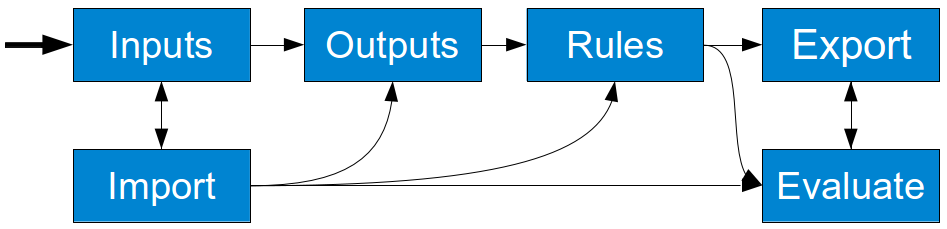
\includegraphics[width=0.6\textwidth]{images/genericPathOne}
\end{center}
\caption{Expected path a user would take through the system}
\label{fig:pathThrough}
\end{figure}
\noindent 
\begin{wrapfigure}[13]{r}{0.395\textwidth}
\hspace{5mm}
\vspace{-10mm}
	\begin{center}
    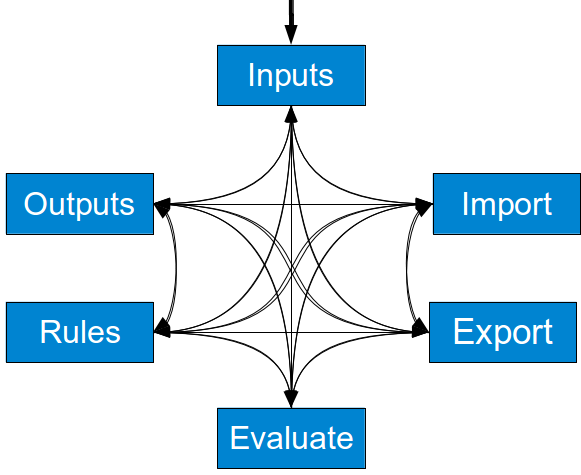
\includegraphics[width=0.41\textwidth]{images/web}
	\end{center}
	\vspace{-7mm}
  \caption{Potential paths that can be taken through the system}
  \vspace{-3mm}
  \label{fig:webThrough}
    \vspace{-13mm}
\end{wrapfigure}
\noindent
Of course, whilst the generally expected path through the system has been determined, this is not the only path through the system, and there is no guarantee that the user will follow this path. In fact, the user has the freedom to traverse the system in any path they please, as shown in figure \ref{fig:webThrough}. This is important for promoting freedom and a sense of control within the system. The user is free to decide how they wish to travel through the system, and this means they are free to traverse forward or backward through the system to make any alterations, or fix any mistakes they may have made.




\newpage 
\subsection{Internal Design}
The user interface of a system is a huge part of the design process, and is extremely important, as this will be how the user will actually be interacting with it. However, this is not the only part of the system that requires designing; as the internal workings of the system also require a lot of thought. \ \\
\ \\
For this project, a web-interface was to be used to interact with a back end that could deal with the processing of a fuzzy logic system. By this point in the project's development, the software's implementation decisions had been made (which are detailed in section \ref{sec:kid}), and the decision of the back end to be used was the FuzzyToolkitUoN R Package, using the R-Shiny service, to interact between the front end and back end. The diagram in figure \ref{fig:architectureDiagram} shows how the interaction between these two systems is handled.

\begin{figure}[ht!]
\begin{center}
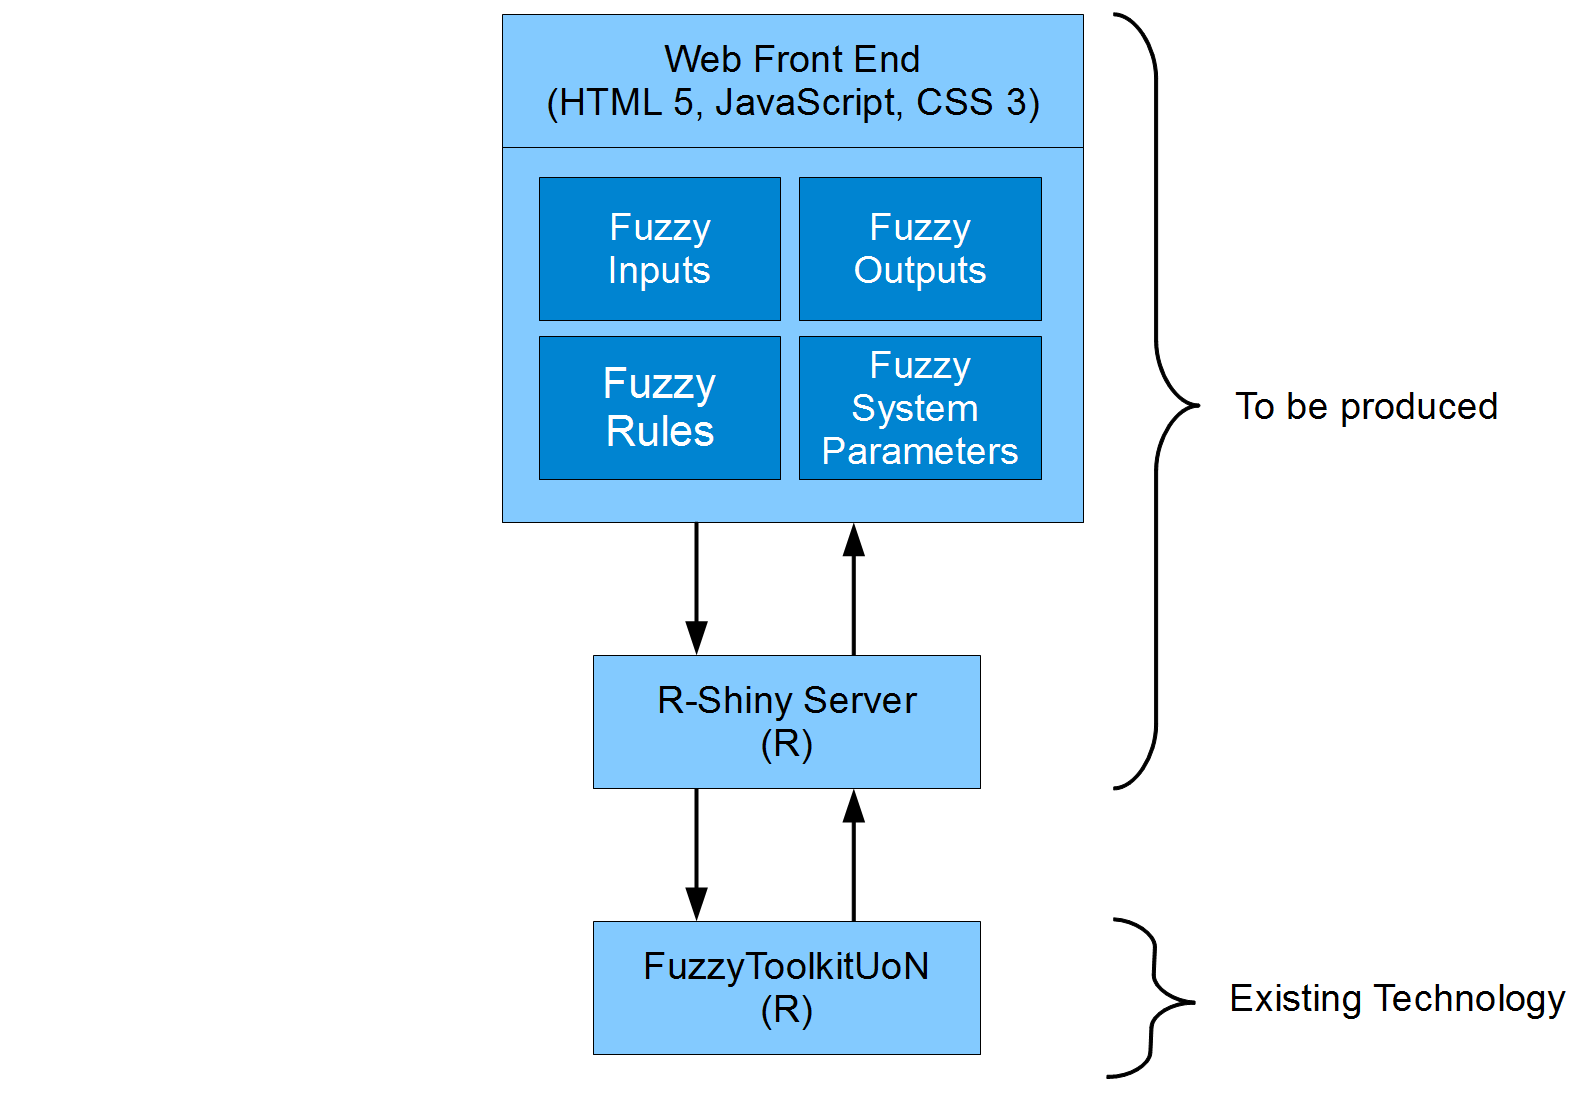
\includegraphics[width=0.9\textwidth]{images/architecture}
\end{center}
\caption{Interaction between the back end and front end of the system}
\label{fig:architectureDiagram}
\end{figure}

\noindent
As you can see, the web front end will be constructed using HTML 5, JavaScript, and CSS 3, and will allow for the creation and specification of fuzzy inputs, outputs, rules, and system parameters. Once a system has been specified, and the user chooses to evaluate the system, the information of the system is passed to the R-Shiny server. This then takes all the form elements from the web front end, extracts their values, and constructs a FIS file, within R. This can then have functions from the FuzzyToolkitUoN package applied to it, and the results of these functions can then be passed back to the web front end, for display to the user.
\newpage 